\documentclass[12pt, a4paper]{article}
\usepackage[utf8]{inputenc}
\usepackage[russian]{babel}
\usepackage[pdftex]{graphicx, color}
\usepackage[left=2cm,right=2cm,top=1.5cm,bottom=2cm]{geometry}
\usepackage{indentfirst}
\usepackage{hyperref}
\usepackage[justification=centering]{caption, subcaption}
\usepackage{amsmath, amsfonts, amssymb, amsthm, amsbsy, mathtools}
\usepackage{mdframed}
\usepackage{setspace}
\usepackage{enumitem}

\usepackage{minted}
\usemintedstyle{tango}
\renewcommand{\listingscaption}{Листинг}

\onehalfspacing

\title{
    
\includegraphics[height=3cm]{pics/msu.png} \\
    \large{
        Отчёт по практическому заданию по курсу <<Суперкомпьютерное моделирование и технологии программирования>> \\
        \textbf{<<Исследование масштабируемости графовых алгоритмов для различных реализаций и различных компьютерных платформ>>}
    }
}
\author{
    \normalsize{Аят Оспанов} \\
    \normalsize{617 группа, ММП, ВМК МГУ, Москва}
}
\date{\normalsize{21 ноября 2017 г.}}

\begin{document}
    \maketitle
    \tableofcontents

    \section{Формулировка задания}
        В данном задании будет исследована масштабируемость графовых алгоритмов на примере \textbf{алгоритма PageRank} из библиотеки \textbf{Parallel Boost Graph Library}. Масштабируемость определяется как зависимость производительности от размеров задачи и числа использованных процессоров (ядер).

        В данном задании предполагается, что графовые алгоритмы оперируют с графами в их простейшем определении: каждый граф -- это совокупность заданного числа вершин и ребер. Графы бывают взвешенные (каждому ребру соответствует некоторое значение) и невзвешенные (каждому ребру соответствует только пара вершин, которые оно соединяет). В случае взвешенного графа каждое ребро определяется как тройка чисел (вершина-начало ребра, вершина-конец ребра, а также вес ребра).

        В качестве основной метрики для оценки производительности целевого компьютера на реализациях графовых алгоритмов используется TEPS (Traversed Edges Per Second) -- число ребер графа, которое алгоритм обходит (обрабатывает) за одну секунду. Для удобства, часто также используются метрики GTEPS и MTEPS с приставками из системы СИ.

        Таким образом, производительность компьютера на реализации графового алгоритма можно вычислить по следующей формуле:
        \begin{gather}
            \text{Производительность(TEPS)}=\frac{\text{число ребер графа}}{\text{время выполнения реализации алгоритма в секундах}}
            \label{eq:teps}
        \end{gather}

        Данная метрика позволяет сравнивать производительность целевого компьютера на реализации графового алгоритма для графов различных размеров, а также для различного числа используемых при вычислениях процессоров. Обычно при увеличении размера графа производительность реализации может заметно снижаться по причине того, что данные перестают попадать в различные уровни кэш-памяти. Данная зависимость крайне интересна, так как графы реального мира имеют всё больший и больший размер, поэтому эффективность реализаций даже для очень больших размеров графов крайне важна. Кроме того, ситуация может меняться и при увеличении числа используемых процессоров.

    \section{Платформа тестирования}
        В качестве платформы для выполнения задания применялся вычислительный комплекс IBM Blue Gene/P.
        \subsection{IBM Blue Gene/P}
            IBM Blue Gene/P -- массивно-параллельная вычислительная система, которая состоит из двух стоек, включающих 8192 процессорных ядер (2 x 1024 четырехъядерных вычислительных узлов), с пиковой производительностью 27,9 терафлопс (27,8528 триллионов операций с плавающей точкой в секунду).

            Характеристики системы:
            \begin{itemize}[leftmargin=1.5cm]
                \item две стойки с вычислительными узлами и узлами ввода-вывода
                \item 1024 четырехъядерных вычислительных узла в каждой из стоек
                \item 16 узлов ввода-вывода в стойке (в текущей конфигурации активны 8, т.е. одна I/O-карта на 128 вычислительных узлов)
                \item выделенные коммуникационные сети для межпроцессорных обменов и глобальных операций
                \item программирование с использованием MPI, OpenMP/pthreads, POSIX I/O
                \item высокая энергоэффективность: ~ 372 MFlops/W (см. список Green500)
                \item система воздушного охлаждения
            \end{itemize}

            Стойка (rack, cabinet) состоит из двух midplane'ов. В midplane входит 16 node-карт (compute node card), на каждой из которых установлено 32 вычислительных узла (compute card). Midplane, 8 x 8 x 8 = 512 вычислительных узлов, -- минимальный раздел, на котором становится доступна топология трехмерного тора; для разделов меньших размеров используется топология трехмерной решетки. Node-карта может содержать до двух узлов ввода-вывода (I/O card). Вычислительный узел включает в себя четырехъядерный процессор, 2 ГБ общей памяти и сетевые интерфейсы.

            Микропроцессорное ядро:
            \begin{itemize}[leftmargin=1.5cm]
                \item модель: PowerPC 450
                \item рабочая частота: 850 MHz
                \item адресация: 32-битная
                \item кэш инструкций 1-го уровня (L1 instruction): 32 KB
                \item кэш данных 1-го уровня (L1 data): 32 KB
                \item кэш предвыборки (L2 prefetch): 14 потоков предварительной выборки (stream \\prefetching): 14 x 256 байтов
                \item два блока 64-битной арифметики с плавающей точкой (Floating Point Unit, FPU), каждый из которых может выдавать за один такт результат совмещенной операции умножения-сложения (Fused Multiply-Add, FMA)
                \item пиковая производительность: 2 FPU x 2 FMA x 850 MHz = 3,4 GFlop/sec per core
            \end{itemize}

            Вычислительный узел:
            \begin{itemize}[leftmargin=1.5cm]
                \item четыре микропроцессорных ядра PowerPC 450 (4-way SMP)
                \item пиковая производительность: 4 cores x 3,4 GFlop/sec per core = 13,6 GFlop/sec
                \item пропускная способность памяти: 13,6 GB/sec
                \item 2 ГБ общей памяти
                \item 2 x 4 МБ кэш-памяти 2-го уровня (в документации по BG/P носит название L3)
                \item легковесное ядро (compute node kernel, CNK), представляющее собой Linux-подобную операционную систему, поддерживающую значительное подмножество Linux-совместимых системных вызовов
                \item асинхронные операции межпроцессорных обменов (выполняются параллельно с вычислениями)
                \item операции ввода-вывода перенаправляются I/O-картам через сеть коллективных операций
            \end{itemize}

    \section{Настройка среды}
        Для выполнения задания требуется библиотека \href{http://www.boost.org/}{\textbf{boost}}. Для выполнения данного задания использовалась библиотека \href{http://www.boost.org/users/history/version_1_47_0.html}{\textbf{boost} версии 1.47}.

        \subsection{Сборка библиотеки boost}
        \begin{enumerate}
            \item Скачивание библиотеки на платформу\\
                \verb|wget --no-check-certificate -c|\\
                \verb|https://sourceforge.net/projects/boost/files/|\\
                $\rightarrow$\verb|boost/1.47.0/boost_1_47_0.tar.gz/download|
            \item Распаковка\\
                \verb|tar -xf boost147_0.tar.gz|
            \item Настройка установщика\\
                \verb|./bootstrap.sh --prefix="../boost_install" --with-toolset=gcc|\\
                \verb|--with-libraries=mpi,filesystem,system,serialization,graph,graph_parallel|
            \item Добавление строк в файл \verb|<boost_root>/tools/build/v2/user-config.jam|:\\
                \verb|using gcc : 4.1.2 : mpicxx : ;|\\
                \verb|using mpi : /bgsys/drivers/ppcfloor/comm/bin/mpicxx ;|
            \item Сборка и установка:\\
                \verb|./b2 --prefix="../boost_install" --layout=versioned|\\
                \verb|toolset=gcc variant=release install|
        \end{enumerate}

        \subsection{Компиляция и запуск программы}\label{sec:compile}
            Компиляция самой программы и вспомогательных программ (будет описано позже) проводилась следующим makefile-ом.
            \inputminted[breaklines=true,fontsize=\scriptsize,frame=single]{make}{makefile}

            Запуск производился следующим bash файлом.
            \inputminted[breaklines=true,fontsize=\scriptsize,frame=single]{bash}{run.sh}

            Где \verb|params.sh|
            \inputminted[breaklines=true,fontsize=\scriptsize,frame=single]{bash}{params.sh}

    \section{Генерация данных}
        Для тестирования были сгенерированы ориентированные невзвешанные графы типа RMAT и SSCA2 с числом вершин $2^{14} - 2^{18}$. Выбор таких размеров был сделан с учетом того, что оперативная память, доступная одному узлу ограничивается 2ГБ, что затрудняет чтение больших файлов, а само чтение производилось из корневого процесса. Генерация файлов производилась с помощью приведенного ниже bash файла, который запускает предварительно скомпилированный с помощью makefile-а (см. раздел \ref{sec:compile}) генератор:
        \inputminted[breaklines=true,fontsize=\scriptsize,frame=single]{bash}{generate.sh}

        Средняя степень связанности каждой вершины, определяющее суммарное число ребер в графе, был оставлен по умолчанию и равна 32. Т.к. мы тестируем алгоритм PageRank, такой выбор был сделан с целью имитации графа сети интернет, который является достаточно разреженным.

    \section{Пример использования библиотечной функции алгоритма PageRank}
        Для исследования алгоритма был написан следующий код, использующий библиотеку boost. Данный код содержит не только запуск алгоритма, но также сбор данных со всех процессов для дальнейшей записи результатов в файл. Данные результаты также пригодятся для проверки корректности результатов работы параллельной версии с последовательной.
        \inputminted[breaklines=true,fontsize=\scriptsize,frame=single]{cpp}{code.cpp}

    \section{Проверка корректности результатов}
        Для проверки корректности результатов был также написан код, использующий последовательную версию алгоритма. Компиляция также производилась с помощью makefile-a: make st (см. раздел \ref{sec:compile}). Запуск проводился с помощью bash файла, приведенного в Приложении (см. Листнг \ref{code:run_st.sh}). Листинг последовательной версии приведен ниже:
        \inputminted[breaklines=true,fontsize=\scriptsize,frame=single]{cpp}{code_st.cpp}

        Также был написан код проверки результатов (см. Листинг \ref{code:check.cpp}) и bash файлы для запуска кода проверки (см. Листинг \ref{code:check.sh}). Нужно добавить, что все версии прошли проверку.

    \section{Исследование масштабируемости}
        По результатам выполнения программы были построены трехмерные графики производительности для двух типов матриц (Рис. \ref{fig:rmat} и Рис. \ref{fig:ssca2}):

        По оси $X$ -- число используемых программой MPI-процессов: 1, 2, 4, 8, 16, 32, 64, 128

        По оси $Y$ -- степень числа вершин графа, от 14 до 18.

        По оси $Z$ -- производительность программы в KTEPS (посчитана по формуле \ref{eq:teps})

        \begin{figure}[h!]
            \centering
            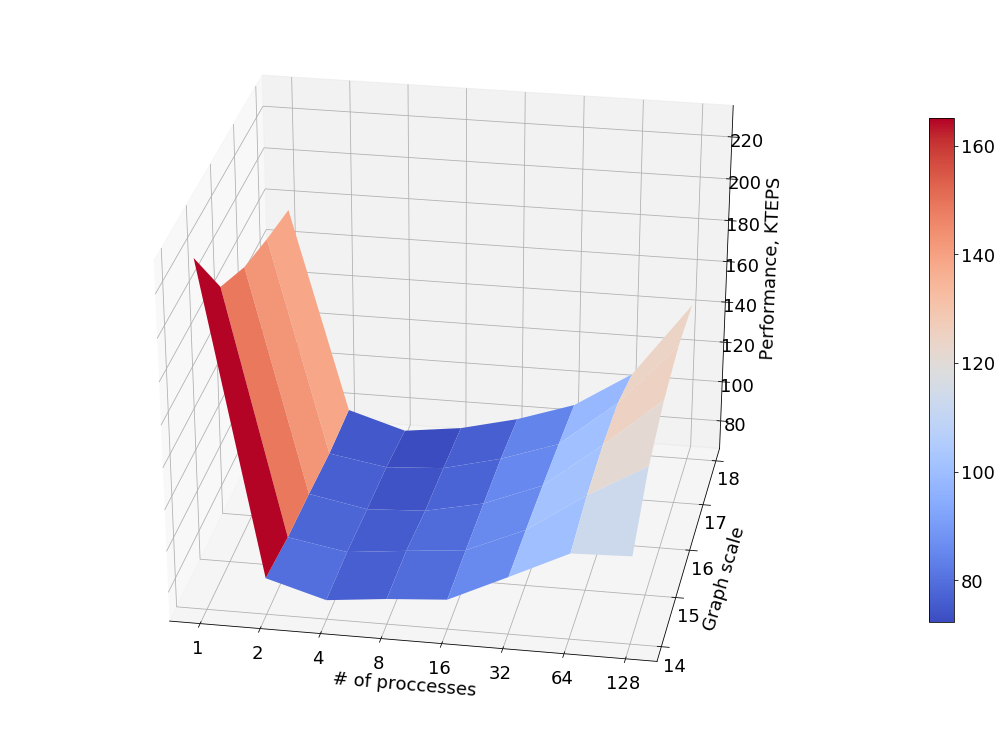
\includegraphics[width=0.9\textwidth]{pics/RMAT}
            \caption{График масштабируемости алгоритма boost::pagerank для графов типа RMAT}
            \label{fig:rmat}
        \end{figure}

        \begin{figure}[h!]
            \centering
            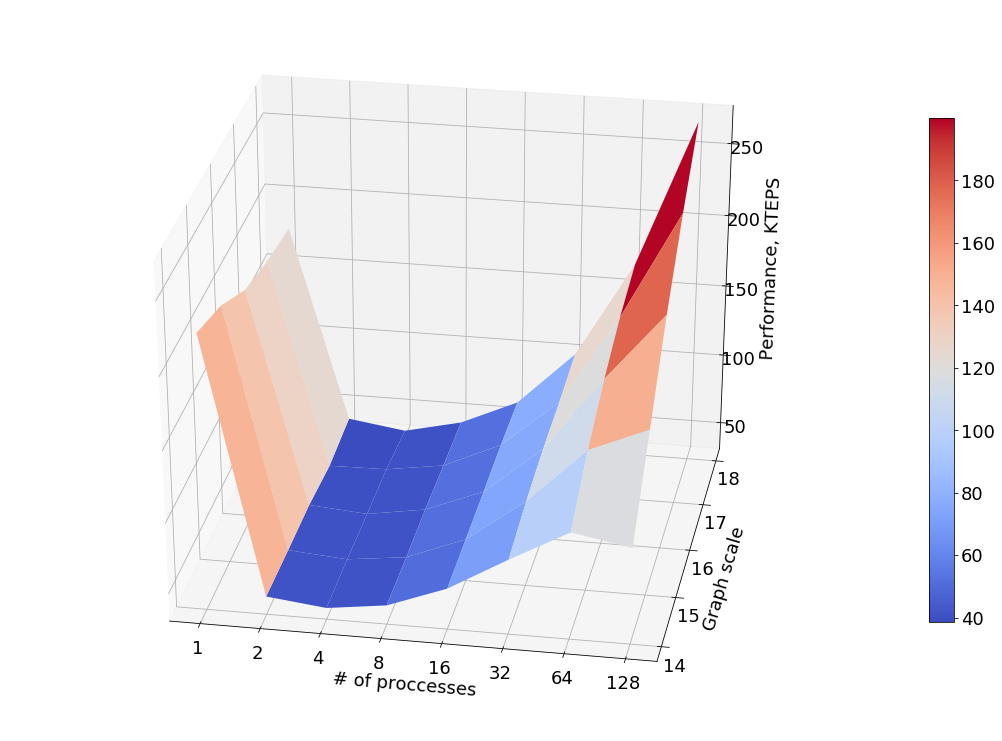
\includegraphics[width=0.9\textwidth]{pics/SSCA2}
            \caption{График масштабируемости алгоритма boost::pagerank для графов типа SSCA2}
            \label{fig:ssca2}
        \end{figure}

    \section{Выводы и результаты}
        Приведенные графики масштабируемости демонстрируют интересные свойства реализации алгоритма. Как видно, на обоих графиках алгоритм показывает достаточно хорошие результаты при одном процессе. Но при двух, резко падает производительность. Хотя начиная с четырех процессов производительность экспоненциально возрастает. Данное поведение можно объяснить следющим образом: т.к. данные помещаются в память одного процесса и нет обмена между процессами, то при одном процессе производительность достаточно хорошая. Начиная с двух процессов начинается обмен данными между процессами, что требует очень много времени. Т.к. при меньших количествах процессов, данных на один процесс приходится много, то увеличивается количество обмениваемых данных. Поэтому, при росте количества процессов, увеличивается производительность. Также можно заметить рост и по размерам графа при количестве процессов больших двух. Объяснить это можно тем, что каждый процесс, при малых количествах данных, не использовался на всю мощь. Это подтверждается и тем, что для одного процесса производительность уменьшается по мере увеличения размера графа.

        Также при сравнении двух графиков можно видеть, что на SSCA2 графе производительность больше, чем на RMAT графе. Это связано со структурами графов. SSCA2 графы имеют независимые компоненты связности, что хорошо подходят для распараллеливания, т.к. обмен между процессами будет меньше, чем в случае с RMAT.

        Для обоих графов по данным графикам нельзя определить глобальные максимумы (доступные аппаратные возможности не позволили это протестировать), т.к. видно, что график растет с ростом количества процессов и степенью графов. Таким образом можно сделать вывод, что алгоритм хорошо распараллеливается. Для данных графиков, максимум для RMAT достигается при 1 процессе и степени вершин 14 (это ни в коем случае нельзя это называть глобальным максимумом), и для SSCA2 -- при 128 процессах и степени вершин графа 18.

    \newpage
    \section{Приложение}
        \begin{listing}[H]
            \caption{Код проверки результатов}
            \label{code:check.cpp}
            \inputminted[breaklines=true,fontsize=\scriptsize,frame=single]{cpp}{check.cpp}
        \end{listing}

        \begin{listing}[H]
            \caption{Код запуска программы проверки}
            \label{code:check.sh}
            \inputminted[breaklines=true,fontsize=\scriptsize,frame=single]{bash}{check.sh}
        \end{listing}

        \begin{listing}[H]
            \caption{Код запуска последовательной программы}
            \label{code:run_st.sh}
            \inputminted[breaklines=true,fontsize=\scriptsize,frame=single]{bash}{run_st.sh}
        \end{listing}
\end{document}
